% Extracted from reviewOfFamousFunctions.tex, problem #3
\begin{problem} \hfil
	\begin{enumerate}
	\item Suppose we're given the right triangle below.  Express $\sin(\theta)$ and $\cos(\theta)$ in terms of the sides of the triangle.

%	\begin{image}
%	\includegraphics[scale=.3]{figure11l.png}
%	\end{image}

\begin{image}[1.5in]
  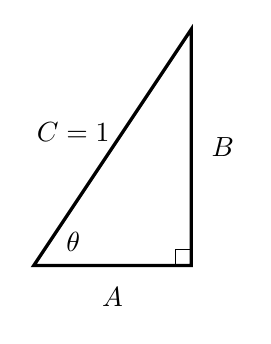
\begin{tikzpicture}
    \coordinate (C) at (0,2);
    \coordinate (D) at (2,2);
    \coordinate (E) at (2,5);
% \tkzMarkRightAngles(C,D,E)
   \tkzMarkAngles(D,C,E)
    \draw[very thick] (D)--(E)--(C)--cycle;
    \draw (1.8, 2) -- (1.8, 2.2) -- (2, 2.2);
    \node at (1,2-.4) {$A$};
    \node at (2.4,3.5) {$B$};
    \node at (1-.5,3.7) {$C=1$};
    \node at (0.5,2.3) {$\theta$};
  \end{tikzpicture}
\end{image}

\WkstHop
	\begin{freeResponse}
	$\sin(\theta)=\frac{B}{C}=B$ and $\cos(\theta)=\frac{A}{C}=A$ 
	\end{freeResponse}

	\item Suppose we are given the triangle below.  
	%	\begin{image}
	%	\includegraphics[scale=.3]{figure22l.png}
	%	\end{image}
\begin{image}[1.5in]
  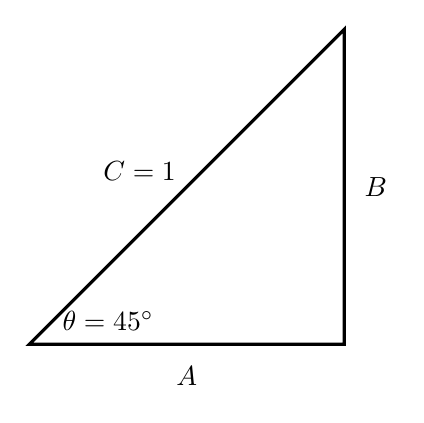
\begin{tikzpicture}
    \coordinate (C) at (0,2);
    \coordinate (D) at (4,2);
    \coordinate (E) at (4,6);
    \tkzMarkRightAngles(C,D,E)
   \tkzMarkAngles(D,C,E)
    \draw[very thick] (D)--(E)--(C)--cycle;
    \node at (2,2-.4) {$A$};
    \node at (4.4,4) {$B$};
    \node at (1+.4,4.2) {$C=1$};
    \node at (1,2.3) {$\theta = 45^\circ$};
  \end{tikzpicture}
\end{image}

		\begin{enumerate}
	\item Find the length of the sides A and B.
\WkstHop
	\begin{freeResponse}
	This is an isosceles triangle. $A=B$  Using the Pythagorean Theorem:
	\begin{align*}
	A^2+B^2&=1^2\\
	2A^2&=1 \\ 	
	A^2&=\frac{1}{2}\\
	A&=\sqrt{\frac{1}{2}}=\frac{\sqrt{2}}{2}\\
	B&=\sqrt{\frac{1}{2}}=\frac{\sqrt{2}}{2}
	\end{align*}
	\end{freeResponse}
	\item Express $\sin\left(\frac{\pi}{4}\right)$ and $\cos\left(\frac{\pi}{4}\right)$ in terms of the sides of the triangle.
\WkstHop
	\begin{freeResponse}
	$\sin\left(\frac{\pi}{4}\right)=\frac{B}{C}=\frac{\sqrt{2}}{2}$ and $\cos\left(\frac{\pi}{4}\right)=\frac{A}{C}=\frac{\sqrt{2}}{2}$

	\end{freeResponse}
	\end{enumerate}
\WkstNew
	\item Suppose we are given the triangle below.  
%		\begin{image}
%		\includegraphics[scale=.5]{figure33l.png}
%		\end{image}
\begin{image}[1.5in]
  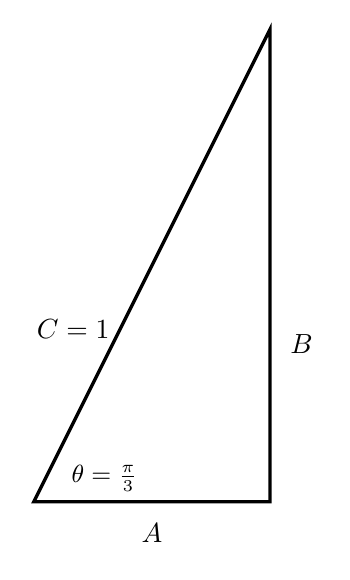
\begin{tikzpicture}
    \coordinate (C) at (0,2);
    \coordinate (D) at (3,2);
    \coordinate (E) at (3,8);
    \tkzMarkRightAngles(C,D,E)
%   \tkzMarkAngle(D,C,E)
    \draw[very thick] (D)--(E)--(C)--cycle;
    \node at (1.5,2-.4) {$A$};
    \node at (3.4,4) {$B$};
    \node at (1-.5,4.2) {$C=1$};
    \node at (0.9,2.3) {\small{$\theta = \frac{\pi}{3}$}};
  \end{tikzpicture}
\end{image}

		\begin{enumerate}
	\item Find the length of the sides A and B.
\WkstHop
	\begin{freeResponse}
	You might remember this as a 30/60/90 triangle.  To find the lengths of the sides of the triangle, we create a triangle as in the figure below.  All the angles in this triangle are of 60 degrees, therefore, this is an equilateral triangle 
		\begin{image}
		\includegraphics[scale=.5]{figure44l.png}
		\end{image}
	Now that we have an equilateral triangle, we have $C=C=2A$.  Thus, $1=2A \implies A=\frac{1}{2}$ \\
	To find B, we use the Pythagorean Theorem.
	\begin{align*}
	\left(\frac{1}{2}\right)^2+B^2&=1^2\\
	\frac{1}{4}+B^2&=1 \\ 	
	B^2&=\frac{3}{4}\\
	B&=\sqrt{\frac{3}{4}}=\frac{\sqrt{3}}{2}
	\end{align*}
	\end{freeResponse}

	\item Express $\sin\left(\frac{\pi}{3}\right)$ and $\cos\left(\frac{\pi}{3}\right)$ in terms of the sides of the triangle.
\WkstHop
	\begin{freeResponse}
	$\sin\left(\frac{\pi}{3}\right)=\frac{B}{C}=\frac{\sqrt{3}}{2}$ and $\cos\left(\frac{\pi}{3}\right)=\frac{A}{C}=\frac{1}{2}$

	\end{freeResponse}
	\end{enumerate}
\WkstNew
\item Suppose we are given the triangle below.  
%		\begin{image}
%		\includegraphics[scale=.5]{figure55l.png}
%		\end{image}
\begin{image}[1.75in]
  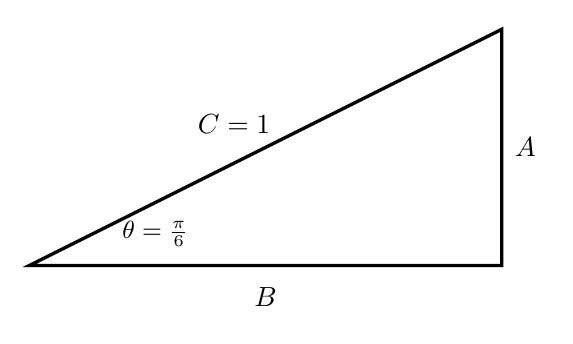
\begin{tikzpicture}
    \coordinate (C) at (0,2);
    \coordinate (D) at (6,2);
    \coordinate (E) at (6,5);
    \tkzMarkRightAngles(C,D,E)
%   \tkzMarkAngle(D,C,E)
    \draw[very thick] (D)--(E)--(C)--cycle;
    \node at (3,1.6) {$B$};
    \node at (6.3,3.5) {$A$};
    \node at (2.6,3.8) {$C=1$};
    \node at (1.6,2.4) {\small{$\theta = \frac{\pi}{6}$}};
  \end{tikzpicture}
\end{image}

		\begin{enumerate}
	\item Find the length of the sides A and B.
\WkstHop
	\begin{freeResponse}
		We've actually already found the lengths of the sides for this type of triangle in part c.  
		$B=\sqrt{\frac{3}{4}}=\frac{\sqrt{3}}{2}$ and $A=\frac{1}{2}$ 
	\end{freeResponse}

	\item Write $\sin\left(\frac{\pi}{6}\right)$ and $\cos\left(\frac{\pi}{6}\right)$ in terms of the sides of the triangle.
\WkstHop
	\begin{freeResponse}
		$\sin\left(\frac{\pi}{6}\right)=\frac{A}{C}=\frac{1}{2}$ and 
		$\cos\left(\frac{\pi}{6}\right)=\frac{B}{C}=\frac{\sqrt{3}}{2}$

	\end{freeResponse}
	\end{enumerate}
\WkstNew
\item 
For any point P(x,y) on the unit circle, we can express its coordinates in terms of $\sin(\theta)$ and $\cos(\theta)$.
Here $\theta$ is the radian measure of the angle in standard position whose terminal side is the line through the origin and the point $P(x,y)$.
\begin{image}
		\includegraphics[scale=.8]{figure1313l.png}
		\end{image}
\WkstHop
		\begin{freeResponse}
			$(x,y)=(\cos(\theta),\sin(\theta))$
		\end{freeResponse}

	\item  Use all of the above information to label the given points on the unit circle.  That is, for each point on the unit circle, provide the angle measure in radians and degrees, and give the (x,y) coordinate for the point.
		\begin{image}
		\includegraphics{figure66l.png}
		\end{image}
\WkstHop

		\begin{freeResponse} \hfil
		\begin{image}
		\includegraphics[scale=.7]{figure77l.png}
		\end{image}
		\end{freeResponse}
	\end{enumerate}

\end{problem}
